\documentclass{article}
\usepackage{tikz}
\usetikzlibrary{shapes,arrows}

\begin{document}

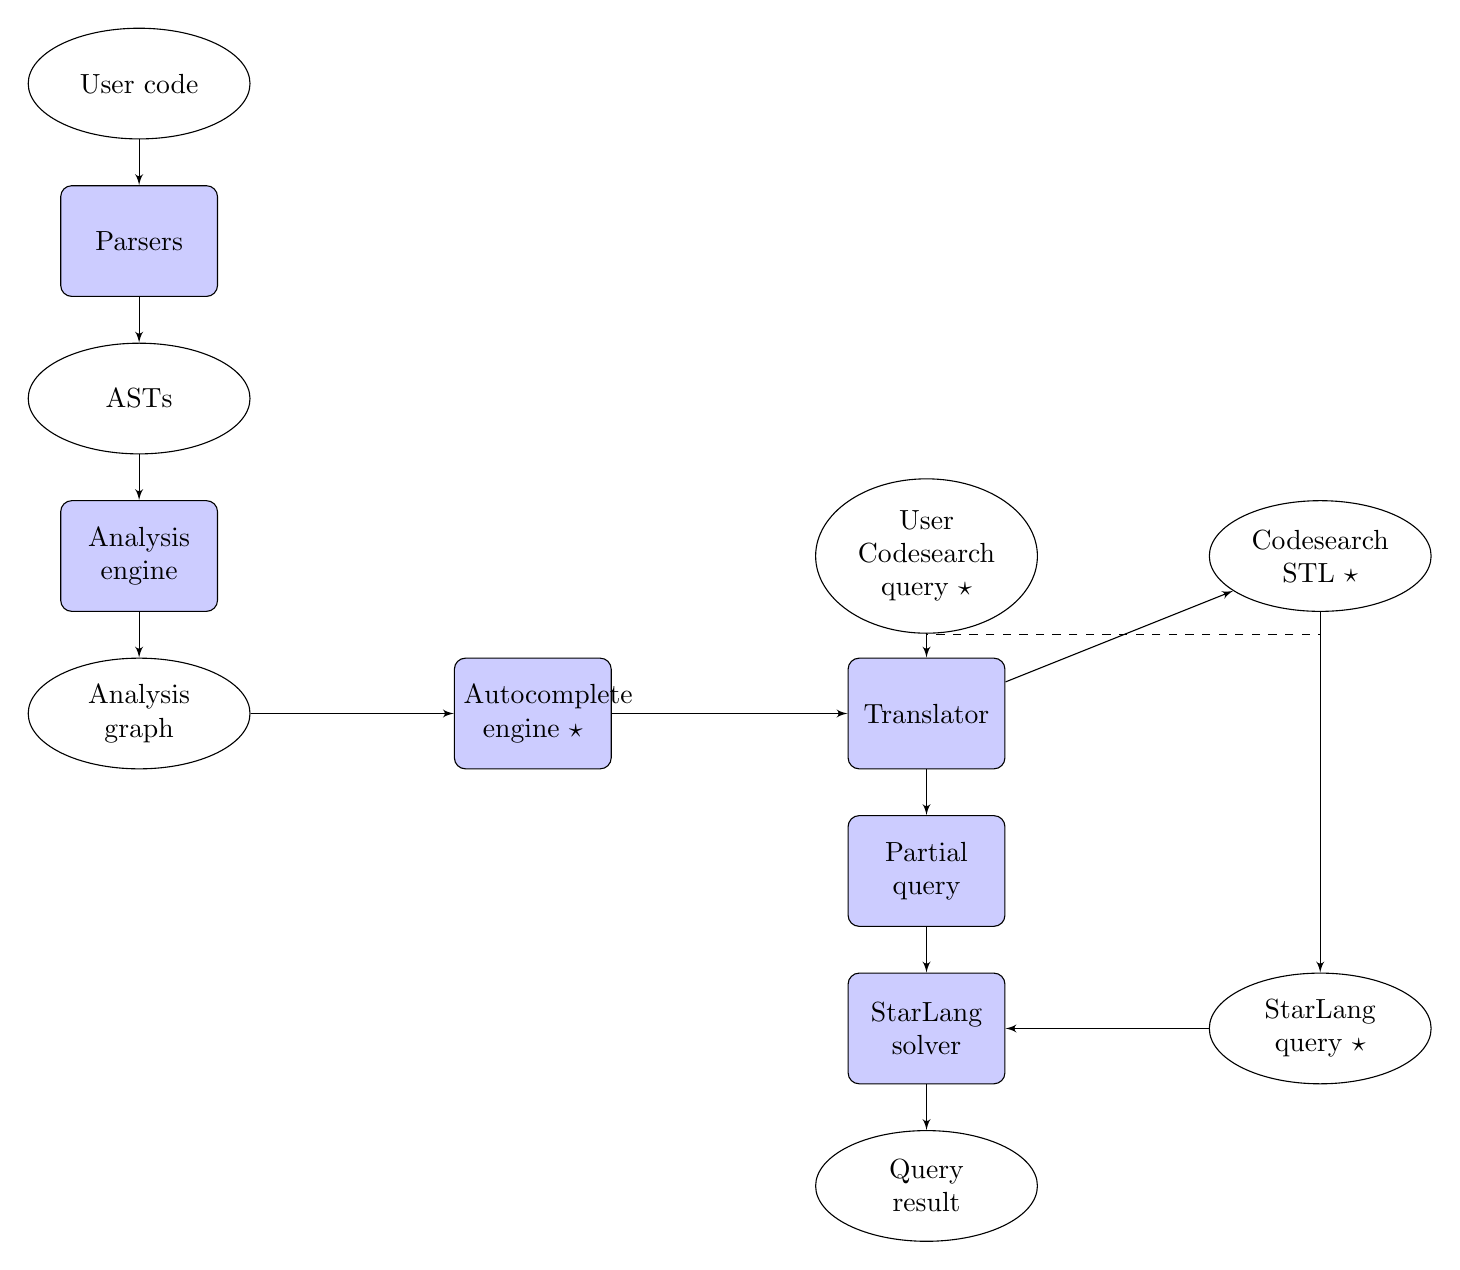
\begin{tikzpicture}[node distance=2cm, auto]
    % Define styles
    \tikzstyle{block} = [rectangle, draw, fill=blue!20, text width=5em, text centered, rounded corners, minimum height=4em]
    \tikzstyle{ellip} = [ellipse, draw, fill=white!20, text width=5em, text centered, rounded corners, minimum height=4em]
    \tikzstyle{line} = [draw, -latex']

    % Nodes
    \node [ellip] (user_code) {User code};
    \node [block, below of=user_code] (parsers) {Parsers};
    \node [ellip, below of=parsers] (asts) {ASTs};
    \node [block, below of=asts] (analysis_engine) {Analysis engine};
    \node [ellip, below of=analysis_engine] (analysis_graph) {Analysis graph};
    \node [block, right of=analysis_graph, xshift=3cm] (auto_complete) {Autocomplete engine $\star$};
    \node [block, right of=auto_complete, xshift=3cm] (translator) {Translator};
    \node [ellip, above of=translator] (user_query) {User Codesearch query $\star$};
    \node [ellip, right of=user_query, xshift=3cm] (stl) {Codesearch STL $\star$};
    \node [block, below of=translator] (partial_query) {Partial query};
    \node [block, below of=partial_query] (starlang_solver) {StarLang solver};
    \node [ellip, right of=starlang_solver, xshift=3cm] (starlang_query) {StarLang query $\star$};
    \node [ellip, below of=starlang_solver] (query_result) {Query result};

    % Draw edges
    \path [line] (user_code) -- (parsers);
    \path [line] (parsers) -- (asts);
    \path [line] (asts) -- (analysis_engine);
    \path [line] (analysis_engine) -- (analysis_graph);
    \path [line] (analysis_graph) -- (auto_complete);
    \path [line] (auto_complete) -- (translator);
    \path [line] (translator) -- (partial_query);
    \path [line] (partial_query) -- (starlang_solver);
    \path [line] (starlang_solver) -- (query_result);
    \path [line] (user_query) -- (translator);
    \path [line] (translator) -- (stl);
    \path [line] (stl) -- (starlang_query);
    \path [line] (starlang_query) -- (starlang_solver);

    % Dashed line
    \draw[dashed] (stl) -- ++(0,-1) -| (user_query);
\end{tikzpicture}

\end{document}